\documentclass[]{article}

\usepackage{graphicx}
\usepackage{placeins}
\usepackage{amsmath,amssymb}
\usepackage[colorlinks=true,citecolor=red]{hyperref}

\usepackage{geometry}
\geometry{a4paper,margin=1in,portrait}

\usepackage{tikz}
\usetikzlibrary{arrows,decorations.pathmorphing,backgrounds,positioning,fit}
\tikzset{module/.style={minimum size = 15mm,rectangle,draw=black,thick,fill=blue!20},
		pre/.style={<-,shorten <=1pt,>=stealth',semithick},
		post/.style={->,shorten <=1pt,>=stealth',semithick}}


\begin{document}
\title{Documentation for digital pattern generator-based imaging controller}
\author{Ryan Thomas}
\date{\today}
\maketitle

\section{Introduction}
\label{sec:introduction}
This document describes the design and operation of the digital pattern generator (DPG)-based imaging controller used in the Kj{\ae}rgaard lab.  While both this controller and its predecessor are implemented using a field-programmable gate array (FPGA), namely the Xlinx Spartan 3AN development board, the DPG imaging controller has a much simpler FPGA architecture and is more easily customizable than the previous, bespoke version.

Whereas the previous imaging controller had many different modules, each of which controlled a different aspect of the timing sequence, the DPG solution has only two modules: the DPG itself and a module to generate triggers for the FlexDDS.  The reason that these are separate is that we need millions of triggers for the FlexDDS at a fixed rate and duty cycle, and using a DPG to generate these would require an enormous amount of memory.  It is easier to use a dedicated module for this purpose.
\begin{figure}[htbp]
	\centering
	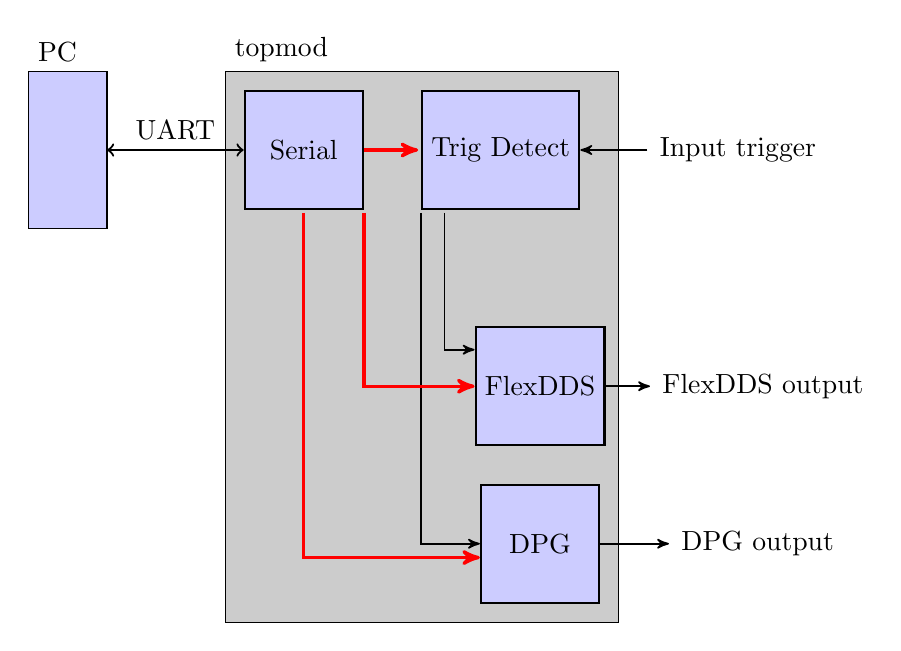
\begin{tikzpicture}
		\draw[fill=black!20] (0,0) rectangle (5,7);
		\node[anchor=south west] (topmod) at (0,7) {topmod};
		\draw[fill=blue!20] (-2.5,5) rectangle (-1.5,7);
		\node[anchor=south west] (pc) at (-2.5,7) {PC};
		\node[module] (serial) at (1,6) {Serial};
		\draw[<->,thick] (-1.5,6) -- node[above] {UART} (serial.west);
%		node[module] (serial) at ++(1,0) {Serial};
%		\node[module] (serial) at (1,6) {Serial} edge[pre] node[anchor=south] {UART} (pc);
		\node[module] (trig-detect) at (3.5,6) {Trig Detect} edge[pre,red,very thick] (serial);
		\node[module] (flexdds) at (4,3) {FlexDDS};
		\node[module] (dpg) at (4,1) {DPG};
		\draw[post] ([xshift=3mm]trig-detect.south west) |- ([yshift=-3mm]flexdds.north west);
		\draw[post] (trig-detect.south west) |- (dpg.west);
		\draw[post,red,very thick] (serial.south east) |- (flexdds.west);
		\draw[post,red,very thick] (serial.south) |- ([yshift=-5]dpg.west);
		
		\node[] (trigin) at ([xshift=2cm]trig-detect.east) {Input trigger} edge[post] (trig-detect.east);
		\node[] (flexdds-out) at ([xshift=2cm]flexdds.east) {FlexDDS output} edge[pre] (flexdds.east);
		\node[] (dpg-out) at ([xshift=2cm]dpg.east) {DPG output} edge[pre] (dpg.east);

	\end{tikzpicture}
	\caption{Diagram of the DPG-based imaging controller. A PC transmits parameters to the FlexDDS trigger generator and a digital pattern to the DPG.  The sequence starts either when an input trigger is received or when a software trigger is issued by the host PC over serial.  Thick red lines indicate the transmission of information to and from the serial controller.}
	\label{fg:diagram}
\end{figure}

\section{Digital Pattern Generator (DPG)}
\label{sec:dpg}
A DPG is simple to understand -- it is a device that stores a list of digital output patterns and the times at which they should be enacted.  In the case of the current DPG, these are stored as a series of 40-bit (5 byte) instructions, where the most-significant byte (MSB) is the type of instruction and bytes 0 to 3 (for a total of 32 bits) are the \emph{data}.  There are currently three types of instructions:
\begin{enumerate}
	\item $\mathrm{MSB} = 0\mathrm{x}00$ This instruction tells the DPG to wait for a time equal to \emph{data} sample clock cycles.
	\item $\mathrm{MSB} = 0\mathrm{x}01$ This instruction tells the DPG to output the pattern equal to \emph{data}.
	\item $\mathrm{MSB} = 0\mathrm{x}02$ This instruction tells the DPG to wait for a digital input event before continuing to the next instruction.  Bits 0 to 3 of \emph{data}, interpreted as an unsigned integer, indicate the digital input channel to look at, and bits 8 to 9 indicate the type of edge to look for.
\end{enumerate}
\begin{figure}
	\centering
	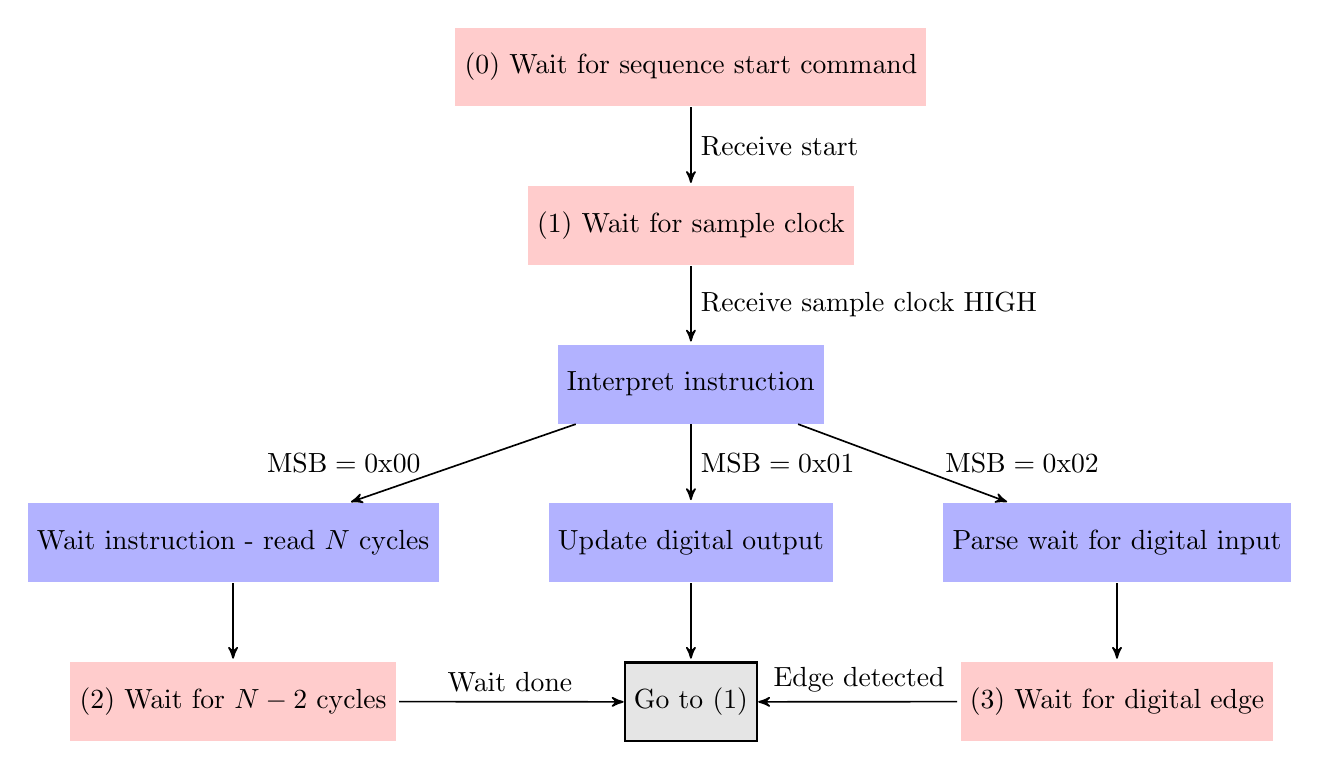
\begin{tikzpicture}[node distance=10mm and 15mm,
		state/.style={rectangle,fill=red!20,minimum size=10mm},
		cond/.style={rectangle,fill=blue!30,minimum size=10mm},
		goto/.style={rectangle,fill=black!10,draw=black,thick,minimum size=10mm}]
		\node[state] (wait-for-start) at (0,0) {(0) Wait for sequence start command};
		\node[state] (wait-for-sample-clock) [below=of wait-for-start] {(1) Wait for sample clock} edge[pre] node[anchor=west] {Receive start} (wait-for-start);
		\node[cond] (interpret-instruction) [below=of wait-for-sample-clock] {Interpret instruction} edge[pre] node[anchor=west] {Receive sample clock HIGH} (wait-for-sample-clock);
		
		\node[cond] (wait) [below left=of interpret-instruction] {Wait instruction - read $N$ cycles} edge[pre] node[left=4mm,anchor=east] {$\mathrm{MSB}=0\mathrm{x}00$} (interpret-instruction);
		\node[state] (wait-for) [below=of wait] {(2) Wait for $N-2$ cycles} edge[pre] node[anchor=east] {} (wait);
		
		\node[cond] (digital-out) [below=of interpret-instruction] {Update digital output}
		edge[pre] node[anchor=west] {$\mathrm{MSB}=0\mathrm{x}01$} (interpret-instruction);
		\node[goto] (goto-1) [below=of digital-out] {Go to (1)} edge[pre] (digital-out);
		\draw[post] (wait-for) -- node[above] {Wait done} (goto-1);
		
		\node[cond,node distance=10mm and 15mm] (wait-input) [below right=of interpret-instruction] {Parse wait for digital input} edge[pre] node[right=4mm,anchor=west] {$\mathrm{MSB}=0\mathrm{x}02$} (interpret-instruction);
		\node[state] (wait-edge) [below=of wait-input] {(3) Wait for digital edge} edge[pre] (wait-input);
		\draw[post] (wait-edge) -- node[above] {Edge detected} (goto-1);
		
%		\node[cond,node distance=10mm and 20mm] (seq-stop) [right=of wait-for-sample-clock] {Sequence stopped} edge[pre] node[anchor=south] {Empty instructions} (wait-for-sample-clock);
%		\draw[post] (seq-stop.north) |- (wait-for-start.east);
	\end{tikzpicture}
	\caption{Diagram of the finite-state machine (FSM) at the heart of the DPG.  Red boxes indicate states of the state machine; blue boxes indicate conditional statements.  New instructions are requested when a ``start'' command is received and also whenever a sample clock HIGH is detected.  When all instructions are read, the FSM returns to state 1.  If a sequence ``stop'' command is received, the controller returns to state 0.}
	\label{fg:dpg}
\end{figure}

At the heart of the DPG is a finite-state machine (FSM) that executes the reads, parses, and executes new instructions: a diagram is shown in Fig.~\ref{fg:dpg}.  The idle state of the DPG is the ``wait-for-start'' state, where the FSM waits for the sequence start command from the PC over the UART (serial) connection.  When it receives this trigger, it raises the \verb|seqEnabled| signal and request a new instruction from the block memory that holds the instruction list.  Raising \verb|seqEnabled| enables the detection of input triggers, and when the input trigger is received the sample clock starts.  The sample clock is set to $1/4$ of the FPGA master clock (but with a duty cycle of $1/4$), so with the current master clock frequency of 100 MHz the sample clock is 25 MHz.  This means that new instructions are processed every 40 ns.  The factor of $1/4$ was chosen to ensure that there is sufficient time to read new instructions from the memory between successive sample clock edges.

When the FSM detects that the sample clock is high it issues a request for a new instruction at the same time that it parses the current one.  When the current instruction number, given by the memory address, is less than the number of stored instructions the FSM also raises the \verb|seqRunning| signal which tells the sample clock generator to continue running.  If the current instruction number is equal to the maximum address, the FSM raises the \verb|seqDone| signal which tells the controller on the next sample clock edge to read the first instruction again and return to the ``wait-for-sample-clock'' state (state 1 in Fig.~\ref{fg:dpg}).  If at any time a ``sequence stop'' command is received, the FSM immediately returns to the idle state (state 0).

If the current instruction is a digital output instruction, the controller routes the \emph{data} part of the instruction to the signal \verb|dOutSig|, which is routed to the physical output when \verb|seqRunning| is high.  If \verb|seqRunning| is low, then the digital output is routed from the signal \verb|dOutManual| which is the manually set value.  This signal can either be a default output state, or the user can set it as needed for testing.  

If the current instruction is a wait instruction, the FSM reads the wait time from \emph{data} as a delay of $N$ sample clock cycles, where $N$ is a 32-bit unsigned integer.  The FSM proceeds to the ``wait'' state (state 2) and waits for $N-2$ cycles - the $-2$ is necessary to account for the sample period during which the instruction is parsed and the periods during which the counting is done.  By choosing to wait for $N-2$, the delays between updates of the digital output are $N$ sample clock cycles.  Note that the controller cannot wait for 0 cycles, and asking it to wait for 1 cycle will result in it waiting for 2 cycles.  In order to have a delay of 1 cycle between successive updates to the digital output, the user should have two successive digital output instructions rather than separating them by a wait time.

Finally, if the current instruction is a wait for input instruction, the FSM reads the input bit from bits 0 to 3 of \emph{data} corresponding to an unsigned integer from 0 to 7.  The edge type to look for is encoded in bits 8 to 9 with a ``00'' being a falling edge, ``01'' being either a falling or rising edge, and ``10'' being a rising edge.  When the correct edge is detected, the FSM moves to state 1.  An edge type of ``11'' is not used and will immediately move to state 1.  Digital inputs are detected synchronously with the master clock, so any input signal must be high for at least one master clock period (10 ns).  

\subsection{Programming the DPG}
\label{sec:programming-dpg}
The DPG is programmed using a relatively simple set of commands which are sent to the FPGA using a serial (UART) connection.  Commands are interpreted least-significant bit (and byte) first.  Some commands set the controller up to read the next command(s) as a numerical parameter, or, in the case of memory uploading, the next series of commands as writes to memory.  A table of commands is given in Table~\ref{tb:commands}
\begin{table}[htbp]
	\centering
	\begin{tabular}{c|c|p{5cm}}
		Command							&	Action													&	Subsequent command(s)\\\hline
		$0\mathrm{xID}\_00\_00\_00$		&	Sequence start											&	None\\\hline
		$0\mathrm{xID}\_00\_00\_01$		&	Sequence stop											&	None\\\hline
		$0\mathrm{xID}\_00\_00\_02$		&	Sends status information back to PC						&	None\\\hline
		$0\mathrm{xID}\_00\_00\_03$		&	Sends current value of \verb|dOutManual| back to PC		&	None\\\hline
		$0\mathrm{xID}\_01\_00\_00$		&	Set value of \verb|dOutManual|							&	Next 32-bit command is interpreted as \verb|dOutManual|\\\hline
		$0\mathrm{xID}\_02\_xx\_xx$		&	Upload instructions to memory - see text				&	Next $0\mathrm{x}00\_00\_xx\_xx$ commands must be 40-bits - see text\\\hline
	\end{tabular}
	\caption{Command options for DPG.  ID is the DPG's serial ID, currently set to $00$.}
	\label{tb:commands}
\end{table}




\end{document}

